\section{Poiseuille flow}
First out for evaluating the LBM solver of the Navier-Stokes equations
is the situation with Poiseuille flow. This is a classic example and
one of the easiest situations were the NS equations are exact
solvable. Consider a 2D channel of length $l$ and width $H$. If the
flow in this channel is driven by a constant force, e.g. a constant
pressure drop, the velocity profile will adopt to a parabolic shape in
the steady state situation. Here follows a brief derivation of the
exact expression for the velocity profile.

Consider the (non-dimensional) Navier-Stokes
eqs. \eqref{eq:lbm:non-dim-ns} and \eqref{eq:lbm:non-dim-massconc} in
2D. Let $x$ be the direction along the channel and $y$ the direction
across the channel. In the case of a pressure gradient in the $x$
direction and no other external forces involved we deduce that the $y$
component of the velocity is zero. Thus eq. \eqref{eq:lbm:non-dim-ns}
reduces to an equation for the $x$ component of the velocity

\begin{equation}
\dfrac{\partial \ux}{\partial t} - \ux \dfrac{\partial \ux}{\partial
  x} = \frac{1}{\Rerm} \dfrac{\partial^2 \ux}{\partial y^2} -
\dfrac{\partial \Prm}{\partial x}.
\end{equation}
 
Under the assumption of a system in a steady state, i.e. ${\partial
  \ux}/{\partial t} = 0$. Further if the flow is fully developed
${\partial \ux}/{\partial x} = 0$, this also assures that
\eqref{eq:lbm:non-dim-massconc} is fulfilled. We now have together
with writing the constant pressure gradient as $\Delta \Prm/l$

\begin{equation}
\dfrac{\partial^2 \ux}{\partial y^2} =
\dfrac{\Rerm\; \Delta\Prm}{l}.
\end{equation}

Solving this eq. with no slip boundary conditions, $\ux(0) = \ux(H) =
0$ gives an expression of the velocity profile

\begin{equation}\label{fig:mb:ana_poi}
\ux(y) = \dfrac{\Rerm\; \Delta\Prm}{2l}y(y - H).
\end{equation}

The benchmark of the LBM solver of the NS equation described in
section \ref{sec:lbm:ns} was performed with a pressure gradient
incorporated as a force. Other possibilities would be to drive the
fluid by imposing fixed pressures/velocities at the inlet and outlet.
In this case, with a driving force, periodic boundary conditions were
imposed at the inlet and outlet. At the channel walls, the bounce-back
boundary condition described in section \ref{lbm:bb} was imposed. The
actual boundary will thus be located half a node-node distance into
the fluid.

A grid with 50 nodes across the channel and 3 in the flow direction
were used. The driving force was set to $\Delta \Prm / l = 1\cdot 10^{-4}$ and
the Reynolds number to $\Rerm = l_0 u_0/\nu$ where the viscosity
is $\nu = 0.2778$ from eq. \eqref{eq:lbm:nu} with $\omega = 0.75$ and
$l_0 = u_0 = 1$. The solution that was obtained after 20000
iterations is presented in fig. \ref{fig:mb:poi}. The analytical
solution, eq. \eqref{eq:mb:ana_poi}, is plotted for comparison.

The agreement between computed and analytical solution is
satisfying. With an RMS error of 9.271$\cdot 10^{-5}$ l.u. and maximum
absolute error of 1.198$\cdot10^{-4}$ l.u.. Note that the actual boundary
is located half a node-node distance into the computational domain,
this is due to the implementation of the bounce-back scheme, see
section \ref{sec:lbm:bb}.  

\begin{figure}
\begin{center}
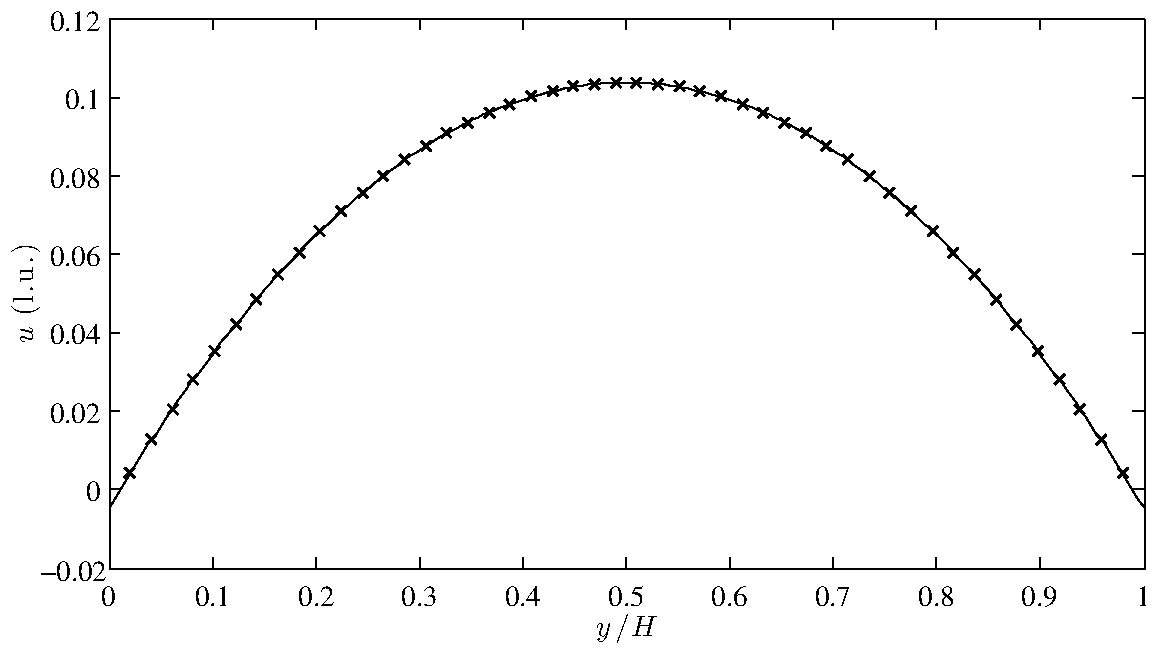
\includegraphics[width=0.9\textwidth]{fig/poiseuille.pdf}
\end{center}
\caption{Obtained velocity profiles of Poiseuille flow ($\times$)
  compared to the analytical solution (solid line). A grid of
  3$\times$50 nodes were used. As expected, there was no variation of
  the velocity field in the flow direction. The velocity is given in
  lattice units.}
\label{fig:mb:poi}
\end{figure}

